\begin{frame}{fragile}
	\frametitle{Features}

\begin{tikzpicture}
    \tikzstyle{obj}=[fill=accentcolor, draw=none, rectangle, minimum width=2.2cm,minimum height=0.8cm];
    \tikzstyle{sobj}=[obj, minimum width=1cm];
    \tikzstyle{link}=[color=accentcolor];
	\begin{scope}[>=stealth]
    
    
    \node(web_interface_image) at (0,0)[draw, circle, color=accentcolor]{
\includegraphics[width=0.0984\textwidth]{images/web-interface-3.png}};
    \node(web_interface_label) [above = 0cm of web_interface_image] {Browser Application};
     
		\pause
		
	    \node(access_control_image) [right = 1.6cm of web_interface_image, draw, circle, color=accentcolor]{
\includegraphics[width=0.08\textwidth]{images/access-control.jpg}};
	    \node(access_control_label) [above = 0cm of access_control_image] {Access Control};
    
	    \pause

		\node(data_types_image) [right = 1.6cm of access_control_image, draw, circle, color=accentcolor]{
\includegraphics[width=0.08\textwidth]{images/data-types.png}};
	    \node(data_types_label) [above = 0cm of data_types_image] {Multiple Data Types};


	    \pause

	    \node(language_binding_image) [right = 1.6cm of data_types_image, draw, circle, color=accentcolor]{
\includegraphics[width=0.1152\textwidth]{images/chain.png}};
	    \node(language_binding_label) [above = 0cm of language_binding_image] {Language Bindings};

    
		\pause

		\node(import_export_image) [below = of web_interface_image, draw, circle, color=accentcolor]{
\includegraphics[width=0.08\textwidth]{images/import-export.png}};
	    \node(import_export_label) [above = 0cm of import_export_image] {Import and Export};
	    
	    \pause

	    \node(fork_image) [right = 1.6cm of import_export_image, draw, circle, color=accentcolor]{
\includegraphics[width=0.08\textwidth]{images/fork.png}};
	    \node(fork_label) [above = 0cm of fork_image] {Fork};

		\pause

	   \node(merge_image) [right = 1.6cm of fork_image, draw, circle, color=accentcolor]{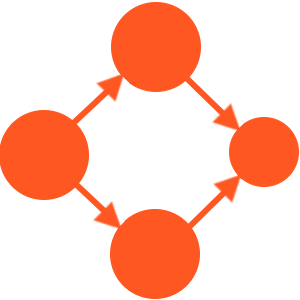
\includegraphics[width=0.08\textwidth]{images/merge.png}};
	   \node(merge_label) [above = 0cm of merge_image] {Merge};

	   \pause

	   \node(diff_image) [right = 1.6cm of merge_image, draw, circle, color=accentcolor]{
\includegraphics[width=0.08\textwidth]{images/diff.png}};
	    \node(diff_label) [above = 0cm of diff_image] {Difference};
	    
    \end{scope}
\end{tikzpicture}


\end{frame}